% $Header: /cvsroot/latex-beamer/latex-beamer/solutions/conference-talks/conference-ornate-20min.en.tex,v 1.6 2004/10/07 20:53:08 tantau Exp $

\documentclass{beamer}

\mode<presentation>
{
%  \usetheme{Hannover}
\usetheme[width=0.7in]{Hannover}
% or ...

  \setbeamercovered{transparent}
  % or whatever (possibly just delete it)
}
\usepackage{longtable}
\usepackage{booktabs}
\usepackage{qtree}

\usepackage[english]{babel}
% or whatever

\usepackage[latin1]{inputenc}
% or whatever

\usepackage{times}
%\usepackage[T1]{fontenc}
% Or whatever. Note that the encoding and the font should match. If T1
% does not look nice, try deleting the line with the fontenc.
%\usepackage{logictheme}

\usepackage{multirow}
\usepackage{totpages}
\usepackage{hyperref}
\usepackage{booktabs}

\usepackage{listings}
\usepackage{tikz}
\usetikzlibrary{positioning}

\newcommand{\blt}{- } %used for bullets in a list

\newcounter{datadefnum} %Datadefinition Number
\newcommand{\ddthedatadefnum}{DD\thedatadefnum}
\newcommand{\ddref}[1]{DD\ref{#1}}

\newcommand{\colAwidth}{0.1\textwidth}
\newcommand{\colBwidth}{0.8\textwidth}

\renewcommand{\arraystretch}{1.1} %so that tables with equations do not look crowded

\pgfdeclareimage[height=0.7cm]{logo}{McMasterLogo}
\title[\pgfuseimage{logo}] % (optional, use only with long paper titles)
{Literate Scientific Software}

%\subtitle
%{Include Only If Paper Has a Subtitle}

\author[Slide \thepage~of \pageref{TotPages}] % (optional, use only with lots of
                                              % authors)
{Spencer Smith, Dan Szymczak  and Jacques Carette}
% - Give the names in the same order as the appear in the paper.
% - Use the \inst{?} command only if the authors have different
%   affiliation.

\institute[McMaster University] % (optional, but mostly needed)
{
  Computing and Software Department\\
  Faculty of Engineering\\
  McMaster University
}
% - Use the \inst command only if there are several affiliations.
% - Keep it simple, no one is interested in your street address.

\date[Jan 12, 2016] % (optional, should be abbreviation of conference name)
{PASC, MS06, June 16, 2016}
% - Either use conference name or its abbreviation.
% - Not really informative to the audience, more for people (including
%   yourself) who are reading the slides online

\subject{computational science and engineering, software engineering, software
  quality, literate programming, software requirements specification, document
  driven design}
% This is only inserted into the PDF information catalog. Can be left
% out. 

% If you have a file called "university-logo-filename.xxx", where xxx
% is a graphic format that can be processed by latex or pdflatex,
% resp., then you can add a logo as follows:

%\pgfdeclareimage[height=0.5cm]{Mac-logo}{McMasterLogo}
%\logo{\pgfuseimage{Mac-logo}}

% Delete this, if you do not want the table of contents to pop up at
% the beginning of each subsection:
% \AtBeginSubsection[]
% {
%   \begin{frame}<beamer>
%     \frametitle{Outline}
%     \tableofcontents[currentsection,currentsubsection]
%   \end{frame}
% }

% If you wish to uncover everything in a step-wise fashion, uncomment
% the following command: 

%\beamerdefaultoverlayspecification{<+->}

\beamertemplatenavigationsymbolsempty 

% have SRS and LP open during the presentation

\begin{document}

%%%%%%%%%%%%%%%%%%%%%%%%%%%%%%%%%%%%%%
\hoffset=-.4in %removing side bar for these frames
\begin{frame}[plain]

\titlepage

\end{frame}
\hoffset=0in %restore
%%%%%%%%%%%%%%%%%%%%%%%%%%%%%%%%%%%%%%

% \begin{frame}

% \frametitle{Literate Scientific Software}
% \tableofcontents
% % You might wish to add the option [pausesections]

% % make like a story - the phases - reason for, why works, advantages
% % changing the history a bit to make a more rational narrative

% \end{frame}

%%%%%%%%%%%%%%%%%%%%%%%%%%%%%%%%%%%%%%

\section[Background]{Background}

% \subsection[Important Software Qualities]{Scientific Computing Software
% Qualities}

%%%%%%%%%%%%%%%%%%%%%%%%%%%%%%%%%%%%%%

\begin{frame}

\frametitle{Important SS Qualities}

\begin{itemize}
\item Reusability
\item Maintainability
\item Verifiability
\item Reproducibility
\end{itemize}

\end{frame}

%%%%%%%%%%%%%%%%%%%%%%%%%%%%%%%%%%%%%%

\begin{frame}

\frametitle{Challenges}

\begin{itemize}
\item Up front requirements
\item Rapid change for numerical algorithms
\item Information duplication
\item Synchronization headaches between artifacts
\item Perceived over-emphasis on non-executable artifacts
%Parnas paper - people do not like docs, vicious cycle
\end{itemize}
\end{frame}

%%%%%%%%%%%%%%%%%%%%%%%%%%%%%%%%%%%%%%

\begin{frame}

\frametitle{``Faked'' Rational Design Process}

\begin{center}
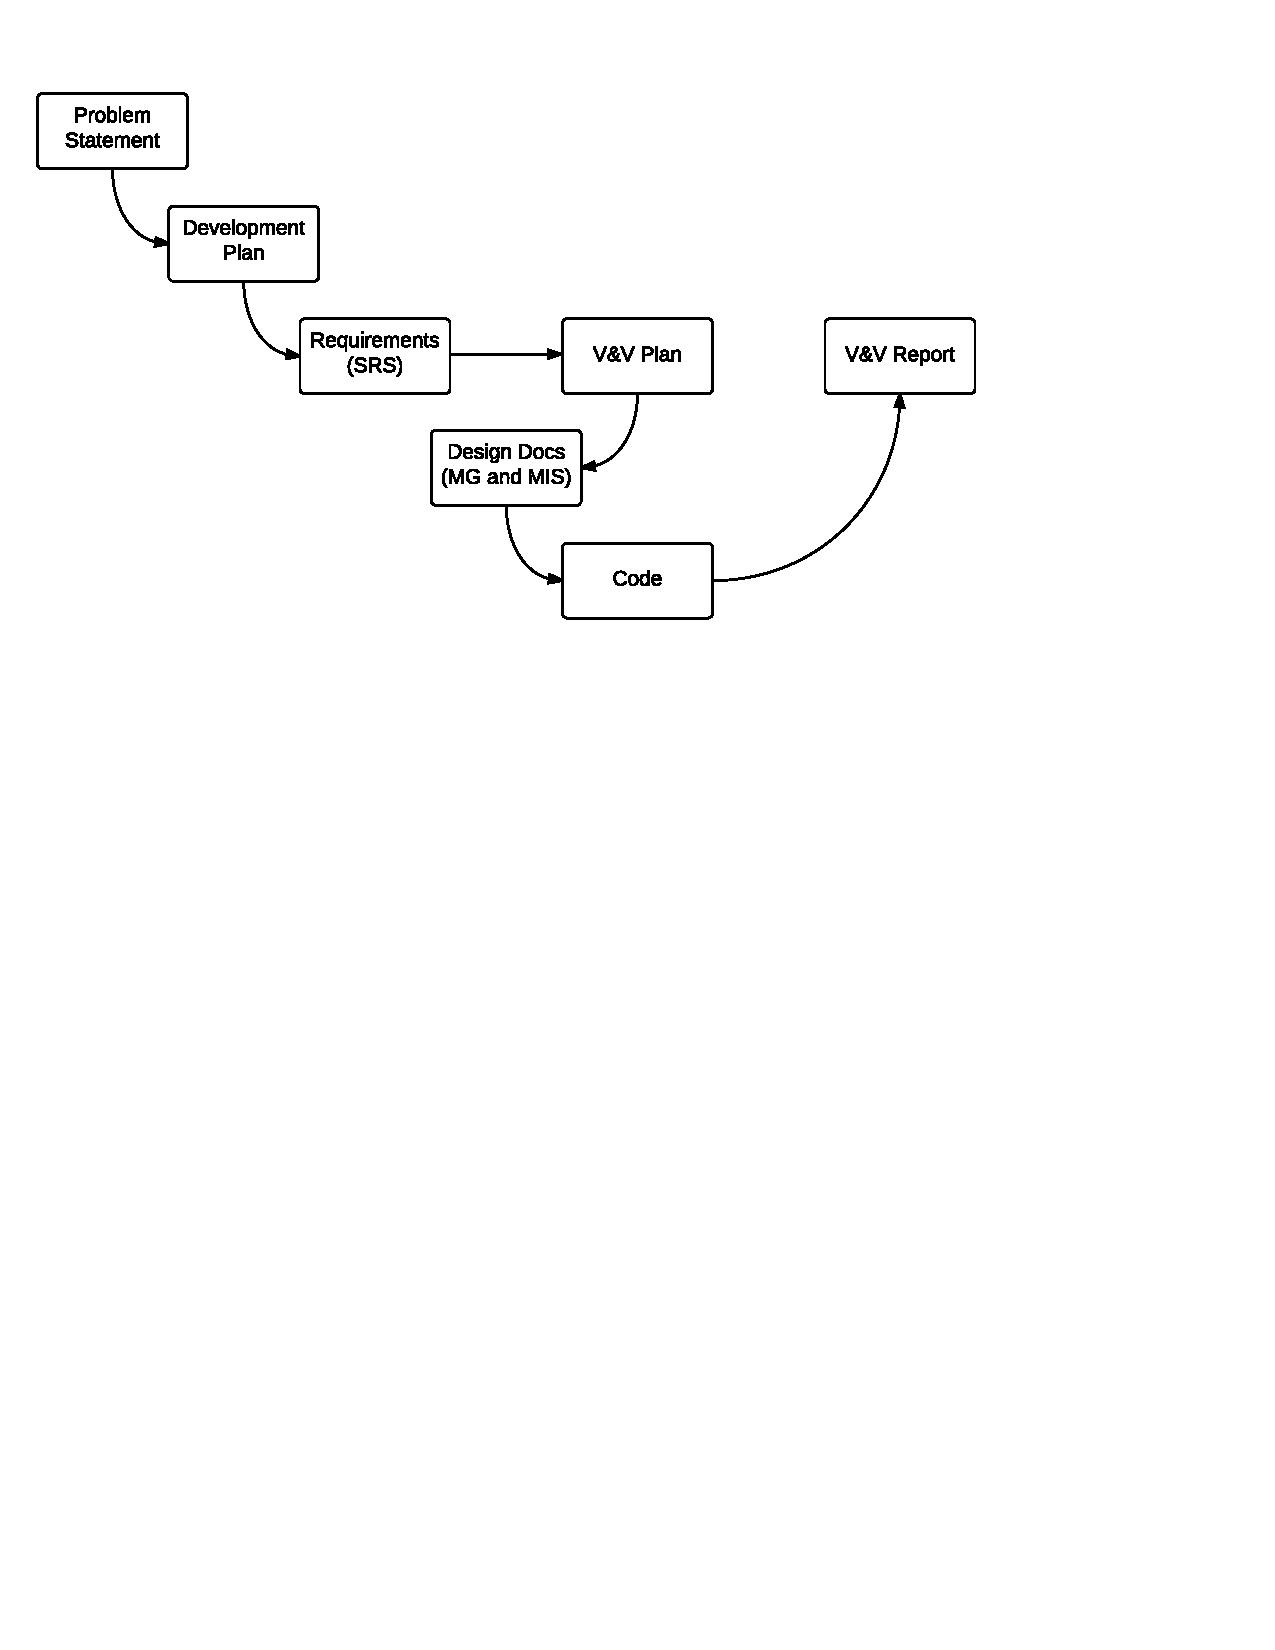
\includegraphics[scale=0.6]{OverviewOfProcess.pdf}
\end{center}

\end{frame}

%%%%%%%%%%%%%%%%%%%%%%%%%%%%%%%%%%%%%%

\begin{frame}

\frametitle{Solar Water Heating Tank}

\begin{center}
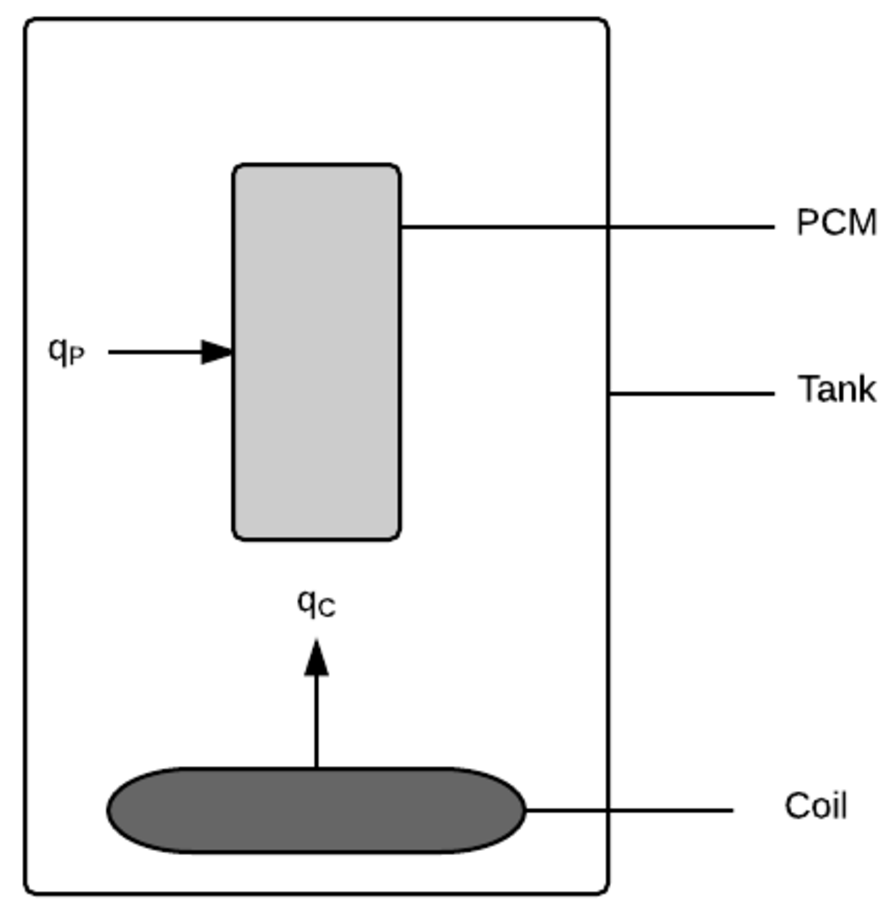
\includegraphics[scale=0.45]{Tank.pdf}
\end{center}

\href{https://github.com/smiths/swhs}{https://github.com/smiths/swhs}

\end{frame}

%%%%%%%%%%%%%%%%%%%%%%%%%%%%%%%%%%%%%%

\section[Lit.\ SS]{Literate Scientific Software}

%%%%%%%%%%%%%%%%%%%%%%%%%%%%%%%%%%%%%%

\begin{frame}

\frametitle{Literate Scientific Software}

\begin{center}
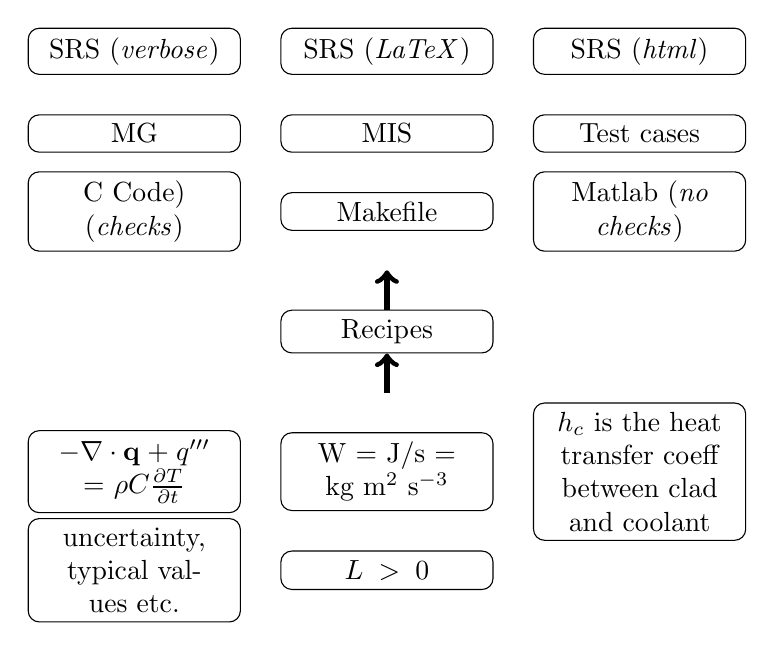
\begin{tikzpicture}[node distance=5mm]
  \tikzstyle{every node}=[draw,shape=rectangle, rounded corners,
    text width=7em, text centered];
  \node (srs)                     	{SRS (\emph{LaTeX})};
  \node (srsh) [right = of srs]  {SRS (\emph{html})};
  \node (srsv) [left = of srs] 	{SRS (\emph{verbose})};
  \node (mis) [below = of srs]       {MIS};
  \node (mg) [left = of mis]       {MG};
  \node (test) [right = of mis]       {Test cases};
  \node (make) [below = of mis]       {Makefile};
  \node (code) [left = of make]       {C Code) (\emph{checks})};
  \node (matlab) [right = of make]       {Matlab (\emph{no checks})};
  \node (recipes) [below = 10mm of make]       {Recipes};
  \node (units) [below = 10mm of recipes]       {W = J/s = kg m$^2$ s$^{-3}$};
  \node (eq) [left = of units]       {$-{\bf \nabla \cdot q} +q'''$ = $\rho C \frac{\partial T}{\partial t}$};
  \node (descipt) [right = of units]       {$h_c$ is the heat transfer coeff between clad and coolant};
  \node (constraint) [below = of units]       {$L > 0$};
  \node (know) [left = of constraint]       {uncertainty, typical values etc.};

  \draw [shorten <=5mm, <-, line width=2pt] (make) -- (recipes);
  \draw [shorten <=5mm, ->, line width=2pt] (units) -- (recipes);
%  \draw [->, line width=2pt] (co.west) -- (-3.56,-1.465) -- (rc); 
		%No idea how to do this
 % \draw [->, line width=2pt] (co) -- (qu);
 % \draw [->, line width=2pt] (co.east) -- (3.56,-1.465) -- (u );
 % \draw [->, line width=2pt] (qu) -- (uc);
 % \draw [->, line width=2pt] (u .south) -- (3.56,-4.58) -- (uc);
 % \draw [->, line width=2pt] (uc) -- (eq);
\end{tikzpicture}
\end{center}

\end{frame}

%%%%%%%%%%%%%%%%%%%%%%%%%%%%%%%%%%%%%%

% \begin{frame}

% \frametitle{Knowledge Based Approach}

% \begin{itemize}
% \item Capture knowledge
% \item From one ``source'' recipes to generate artifacts
% \item Automated
% \item Inspired by Knuth's Literate Programming
% \end{itemize}
% \end{frame}

%%%%%%%%%%%%%%%%%%%%%%%%%%%%%%%%%%%%%%

\begin{frame}

\frametitle{How LSS Addresses Challenges}

\begin{itemize}
\item Supports changing requirements and design
\begin{itemize}
\item Generation
\item Automated traceability
\end{itemize}
\item Supports duplication 
\begin{itemize}
\item Knowledge is entered once, generated/transformed% as required
\item Eases maintenance
\item If incorrect, incorrect everywhere
\end{itemize}
\item Non-executable artifacts are generated
\end{itemize}
\end{frame}

%%%%%%%%%%%%%%%%%%%%%%%%%%%%%%%%%%%%%%

\begin{frame}

\frametitle{Verifiability}

\begin{table} 
\centering
%\caption{Constraints on quantities}
\begin{tabular}{c c r c } 
\toprule
\textbf{Var} & \textbf{Constraints} & \textbf{Typical Value} & \textbf{Uncertainty}\\ \midrule
$L$ & $L > 0$ & 1.5 m & 10\% \\ 
$D$ & $D > 0$ & 0.412 m & 10\% \\ 
$V_P$ & $V_P > 0$ & 0.05 m$^3$	& 10\% \\
$A_P$ & $A_P > 0$ & 1.2 m$^2$	& 10\% \\
$\rho_P$ & $\rho_P > 0$	& 1007 kg/m$^3$	& 10\% \\
\bottomrule
\end{tabular}
\label{tab:pcm}
\end{table}

\begin{equation*}
E_W = \int_{0}^{t} h_C A_C (T_C - T_W(t)) dt - \int_{0}^{t} h_P A_P (T_W(t) - T_P(t)) dt
\end{equation*}

\begin{itemize}
\item Sanity checks captured and reused
\item Generate guards against invalid input
\item Generate test cases
\end{itemize}
\end{frame}

%%%%%%%%%%%%%%%%%%%%%%%%%%%%%%%%%%%%%%

\begin{frame}

\frametitle{Reusability}

\noindent
\begin{minipage}{\columnwidth}
\begin{tabular}{@{} p{\colAwidth}  p{\colBwidth}@{}}
\toprule
\textbf{Num.}& \textbf{T1} \\
\midrule
Label &\bf Conservation of energy\\
\midrule
Eq &  $-{\bf \nabla \cdot q} +q'''$ = $\rho C \frac{\partial T}{\partial t}$ \smallskip\\
\midrule
Descrip & The above equation gives the conservation of energy for time 
varying heat transfer in a material of specific heat capacity $C$ and density $\rho$,
where $\bf q$ is the thermal flux vector, $q'''$ is the volumetric heat
generation, $T$ is the temperature, $\nabla$ is the del operator and $t$ is the time.\\
\bottomrule
\end{tabular}
\end{minipage}

\end{frame}

%%%%%%%%%%%%%%%%%%%%%%%%%%%%%%%%%%%%%%

\begin{frame}

\frametitle{Maintainability}

\begin{itemize}

\item[A1:] The
  only form of energy that is relevant for this problem is thermal energy.  All
  other forms of energy, such as mechanical energy, are assumed to be
  negligible [T1].

\item[A2:] All heat transfer coefficients are constant over time [GD1].

\item[A3:] The water in
  the tank is fully mixed, so the temperature is the same throughout the entire
  tank [GD2, DD2].

\item[A4:] The PCM has the same temperature throughout [GD2, DD2, LC1].

\item[A5:] etc.

\end{itemize}

\end{frame}

%%%%%%%%%%%%%%%%%%%%%%%%%%%%%%%%%%%%%%

\begin{frame}

\frametitle{Reproducibility}

\begin{itemize}
\item Knowledge is explicitly stored for the future
\item Recipes used to regenerate all artifacts, not just code or results
\item Recipes include build instructions
\end{itemize}
\end{frame}

%%%%%%%%%%%%%%%%%%%%%%%%%%%%%%%%%%%%%%

% \begin{frame}

% \frametitle{Software Certification}

% \begin{itemize}
% \item Recertification can be expensive and time consuming
% \item Change propagates through documentation
% \item Traceability and maintainability
% \item Recipes help with changing documentation standards
% \end{itemize}

% \end{frame}

%%%%%%%%%%%%%%%%%%%%%%%%%%%%%%%%%%%%%%

\section[Drasil]{Drasil}

%%%%%%%%%%%%%%%%%%%%%%%%%%%%%%%%%%%%%%

\begin{frame}

\frametitle{Drasil Framework Design}

\begin{center}
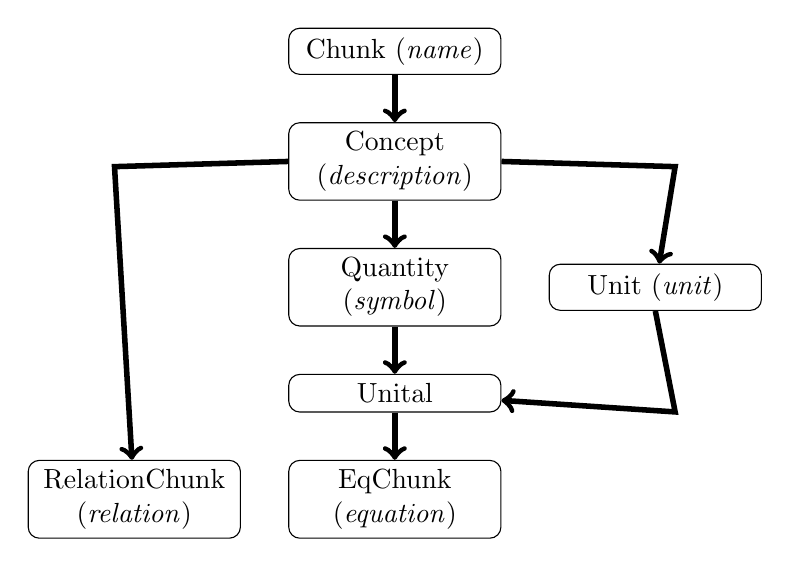
\begin{tikzpicture}[node distance=6mm]
  \tikzstyle{every node}=[draw,shape=rectangle, rounded corners,
    text width=7em, text centered];
  \node (ch)                     	{Chunk (\emph{name})};
  \node (co) [below = of ch]       {Concept (\emph{description})};
  \node (qu) [below = of co]  		{Quantity (\emph{symbol})};
  \node (u ) [right = of qu] 		{Unit (\emph{unit})};
  \node (uc) [below = of qu] 		{Unital};
  \node (eq) [below = of uc]	{EqChunk (\emph{equation})};
  \node (rc) [left = of eq]	{RelationChunk (\emph{relation})};

  \draw [->, line width=2pt] (ch) -- (co);
  \draw [->, line width=2pt] (co.west) -- (-3.56,-1.465) -- (rc); 
		%No idea how to do this
  \draw [->, line width=2pt] (co) -- (qu);
  \draw [->, line width=2pt] (co.east) -- (3.56,-1.465) -- (u );
  \draw [->, line width=2pt] (qu) -- (uc);
  \draw [->, line width=2pt] (u .south) -- (3.56,-4.58) -- (uc);
  \draw [->, line width=2pt] (uc) -- (eq);
\end{tikzpicture}
\end{center}

\end{frame}

%%%%%%%%%%%%%%%%%%%%%%%%%%%%%%%%%%%%%%

\begin{frame}[fragile]

\frametitle{Simple SRS from LaTeX}

\href{run:SRS.pdf}{SRS from LaTeX}

\end{frame}

%%%%%%%%%%%%%%%%%%%%%%%%%%%%%%%%%%%%%%

\hoffset=-.8in %removing side bar for these frames

\begin{frame}[plain, fragile]

%\frametitle{Example Recipe}

\begin{lstlisting}[frame=none, 
  showstringspaces=false, basicstyle=\footnotesize]
vars :: [EqChunk]
vars = [h_g, h_c]

s1, s2, s3, s4 :: LayoutObj
s1=table_of_units si_units
s2=table_of_symbols vars
s3=Section 0 (S "Data Definitions") $ map (Definition.Data) vars
s4=Section 0 (S "Code") $ map (CodeBlock.toCode CLang Calc) [h_c]

srs :: Quantity s => [s] -> String -> [LayoutObj] -> Document
srs ls author body =
  Document ((S "SRS for ") :+: 
    (foldr1 (:+:) (intersperse (S " and ") 
    (map (\x -> U $ x ^. symbol) ls))))
    (S author) body  
  
srsBody :: Document
srsBody = srs vars "Spencer Smith" [s1, s2, s3, s4]
\end{lstlisting}
\end{frame}

\hoffset=0in %resetting side bar
%%%%%%%%%%%%%%%%%%%%%%%%%%%%%%%%%%%%%%

\hoffset=-.8in %removing side bar for these frames

\begin{frame}[plain, fragile]

%\frametitle{Example Recipe}

\begin{lstlisting}[frame=none, showstringspaces=false, basicstyle=\footnotesize]

table_of_symbols :: (Unit s, Quantity s) => [s] -> LayoutObj
table_of_symbols ls=Section 0 (S "Table of Sym") [intro,table ls]

intro :: LayoutObj
intro = Paragraph $ 
  S "The table that follows ..."
  
table :: (Unit s, Quantity s) => [s] -> LayoutObj
table ls=Table [S "Symbol",S "Description",S "Units"] (mkTable
  [(\ch -> U (ch ^. symbol)), 
   (\ch -> ch ^. descr), 
   (\ch -> Sy $ ch ^. unit)] ls)
  (S "Table of Symbols") False

\end{lstlisting}
\end{frame}

\hoffset=0in %resetting side bar
%%%%%%%%%%%%%%%%%%%%%%%%%%%%%%%%%%%%%%

\hoffset=-.8in %removing side bar for these frames

\begin{frame}[plain, fragile]

%\frametitle{Example Recipe}

\begin{lstlisting}[frame=none, showstringspaces=false, basicstyle=\footnotesize]

fundamentals :: [FundUnit]
fundamentals = [metre, kilogram, second, ...]

derived :: [DerUChunk]
derived = [centigrade, joule, watt, calorie, kilowatt]

si_units :: [UnitDefn]
si_units = map UU fundamentals ++ map UU derived

------------- Fundamental SI Units ---------------------------------------------
fund :: String -> String -> String -> FundUnit
fund nam desc sym = UD (CC nam (S desc)) (UName $ Atomic sym)

metre, kilogram, second, ... :: FundUnit
metre    = fund "Metre"    "length"               "m"
kilogram = fund "Kilogram" "mass"                 "kg"
second   = fund "Second"   "time"                 "s"
kelvin   = fund "Kelvin"   "temperature"          "K"
mole     = fund "Mole"     "amount of substance"  "mol"
ampere   = fund "Ampere"   "electric current"     "A"
candela  = fund "Candela"  "luminous intensity"   "cd"

\end{lstlisting}
\end{frame}

\hoffset=0in %resetting side bar

%%%%%%%%%%%%%%%%%%%%%%%%%%%%%%%%%%%%%%

\hoffset=-0.8in %no side bar
\begin{frame}[plain, fragile]

%\frametitle{The $h_c$ Chunk}

$$h_{c} = \frac{2k_{c} h_{b}}{2k_{c}+\tau_{c}h_{b}}$$

\begin{lstlisting}[frame=none, showstringspaces=false, basicstyle=\footnotesize]

heat_transfer :: DerUChunk
heat_transfer = DUC (UD ht_con ht_symb) heat_transfer_eqn

ht_con :: ConceptChunk
ht_con = makeCC "Heat transfer" "Heat transfer"

ht_symb :: USymb
ht_symb = from_udefn heat_transfer_eqn

heat_transfer_eqn = USynonym (UProd 
  [kilogram ^. unit, UPow (second ^. unit) (-3),
   UPow (centigrade ^. unit) (-1)])

h_c_eq :: Expr
h_c_eq = 2*(C k_c)*(C h_b)/(2*(C k_c)+(C tau_c)*(C h_b))

h_c :: EqChunk
h_c = fromEqn "h_c" (S "convective heat transfer ...") 
  (lH `sub` lC) heat_transfer h_c_eq

\end{lstlisting}

\end{frame}

\hoffset=0in %resetting side bar

%%%%%%%%%%%%%%%%%%%%%%%%%%%%%%%%%%%%%%

\section[Next Steps]{Next Steps}

%%%%%%%%%%%%%%%%%%%%%%%%%%%%%%%%%%%%%%

\begin{frame}

\frametitle{Next Steps: Design Documentation}

\begin{center}
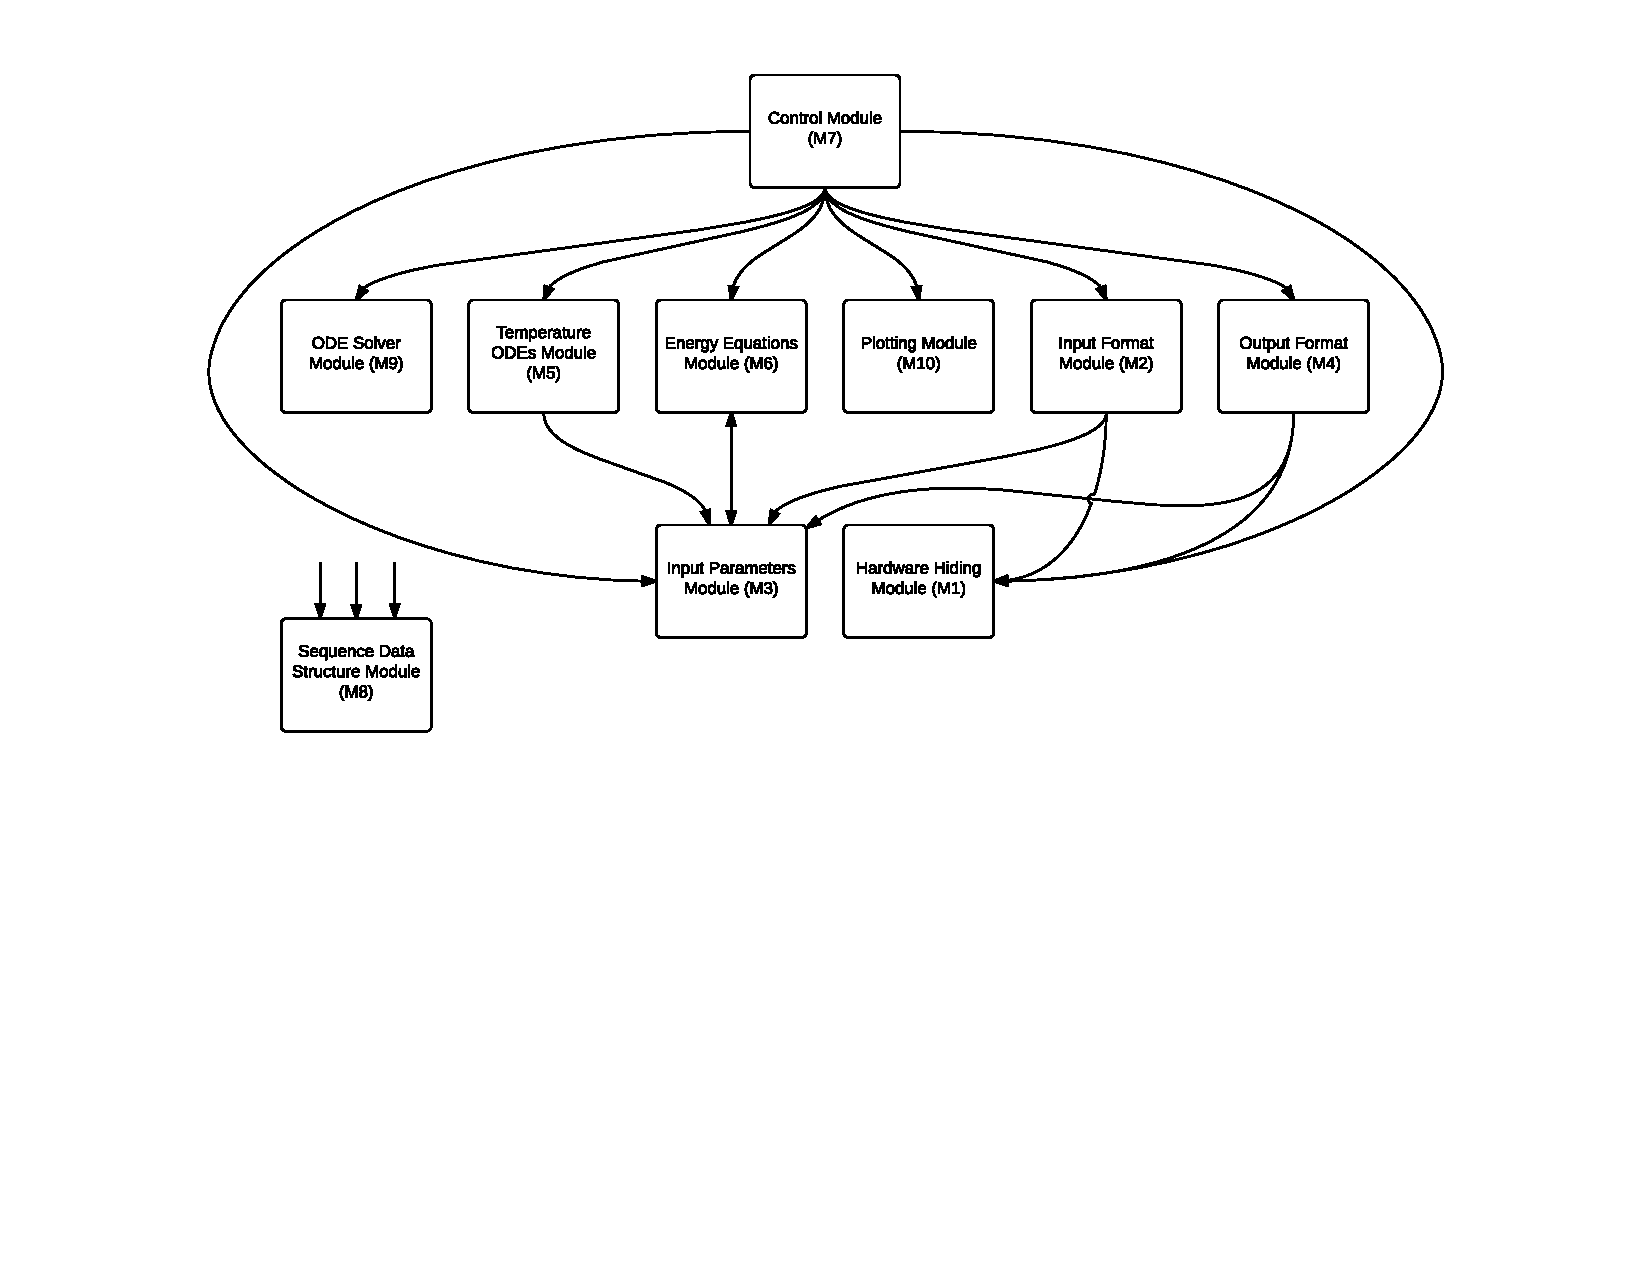
\includegraphics[scale=0.47]{UsesHierarchy.pdf}
\end{center}

\end{frame}

%%%%%%%%%%%%%%%%%%%%%%%%%%%%%%%%%%%%%%

\begin{frame}

\frametitle{Generate Code for IMs}

\noindent
\begin{minipage}{\columnwidth}
\begin{tabular}{@{} p{\colAwidth}  p{\colBwidth}@{}}
\toprule
% \textbf{Number}& \textbf{IM2} \\
% \midrule
% Label & \bf Energy balance on PCM to find $T_P$\\
% \midrule
Input&  $m_P$, $C_P^S$, $C_P^L$, $h_P$, $A_P$, $t_\text{final}$, $T_\text{init}$, $T_\text{melt}^P$,
$T_W(t)$ from IM1\\
\midrule
Output & $T_P(t)$, $0 \leq t \leq t_\text{final}$, with initial 
conditions, $T_W(0) = T_P(0) = T_\text{init}$ (A12), and $T_W(t)$ 
from IM1, such that the following governing ODE is satisfied.  The
specific ODE depends on $T_P$ as follows:\\
&  $
  \frac{dT_P}{dt} = \begin{cases}
  \frac{dT_P}{dt} = \frac{1}{\tau^S_P}(T_W(t) - T_P(t)) & \text { if } T_P<T_\text{melt}^P\\
  \frac{dT_P}{dt} = \frac{1}{\tau^L_P}(T_W(t) - T_P(t)) & \text { if } T_P>T_\text{melt}^P\\
  0 & \text { if }  T_P=T_\text{melt}^P \\
   ~ & \text{ and } 0 < \phi < 1\\
  \end{cases}
  $
\\
\bottomrule
\end{tabular}
\end{minipage}

\end{frame}

%%%%%%%%%%%%%%%%%%%%%%%%%%%%%%%%%%%%%%

\begin{frame}

\frametitle{Approach to Developing Drasil}

\begin{itemize}
\item Case studies
\begin{itemize}
\item Solar water heating tank
\item Slope stability analysis
\item Glass safety analysis
\item Game physics engine
\end{itemize}
\item Practical
\item Not trying to automate everything %trust developer
\item Small chunks of knowledge
\item Look for patterns
\item Attempt to capture design decisions
\begin{itemize}
\item Version control
\item Issue tracking
\end{itemize}
\end{itemize}

\end{frame}

%%%%%%%%%%%%%%%%%%%%%%%%%%%%%%%%%%%%%%

\section[Conclusions]{Conclusions}

%%%%%%%%%%%%%%%%%%%%%%%%%%%%%%%%%%%%%%

\begin{frame}

\frametitle{Concluding Remarks}

\begin{itemize}
\item SS has the opportunity to lead other software fields by leveraging its
  solid existing knowledge base
\item Document driven design is feasible with a knowledge-based approach
\item Documentation for QA and software certification does not have to be
  painful, expensive or time consuming
\item Drasil will be developed via practical case studies
\end{itemize}
\end{frame}

%%%%%%%%%%%%%%%%%%%%%%%%%%%%%%%%%%%%%%

\end{document}